\documentclass[aspectratio=169]{beamer}
\usepackage{standalone}
\usepackage{amsmath}
\usepackage{bm}

\usepackage{stmaryrd}
\usepackage{listings}
\usepackage{bussproofs}

\usepackage[hyperref=auto,style=alphabetic,backend=bibtex]{biblatex}
\addbibresource{kwarcpubs.bib}
\addbibresource{extpubs.bib}
\addbibresource{extcrossrefs.bib}
\addbibresource{bib.bib}
\usepackage{appendixnumberbeamer}
\usepackage{tikz}
\usepackage{tikz-qtree}
\usetikzlibrary{arrows.meta}

\usetheme{Pittsburgh}
% \setbeamertemplate{footline}[frame number]
\setbeamertemplate{footline}{\hfill\insertframenumber\,/\,\inserttotalframenumber\quad\strut}
\setbeamertemplate{navigation symbols}{}
\usecolortheme{beaver}
\setbeamertemplate{frametitle}[default][left]
% \setbeamersize{text margin left=3em}

\usepackage{utils/colors}
\usepackage[forbeamer]{utils/basic}
\usepackage{utils/operators}
\usepackage{utils/mylstmisc}
\usepackage{utils/lstmmt}

% \lstset{basicstyle=\ttfamily}
% \lstset{commentstyle=\itshape\color{commentfont}}
% \definecolor{codegray}{rgb}{0.9,0.9,0.9}
\lstset{basicstyle=\sf,columns=fullflexible}
\lstset{numberstyle=\tiny}
\lstset{language={[LaTeX]TeX}}
\lstset{literate=--1}

\title{Semantic Authoring in a Flexiformal Context --- Bulk Annotation of Rigorous Documents}

\author{Michael Kohlhase, \bf Jan Frederik Schaefer}
\institute{FAU Erlangen-N\"urnberg}
\date{18\textsuperscript{th} Conference on Intelligent Computer Mathematics\\Brasilia, Brazil\\October 8, 2025}

        

\begin{document}

\frame\titlepage


\begin{frame}
    \frametitle{ALeA ecosystem}
    \begin{columns}
        \column{0.4\textwidth}
        An adaptive learning assistant that
        \begin{itemize}
            \item tracks learner's progress,
            \item suggests practice problems,
            \item is powered by semantic annotations.
        \end{itemize}
        \column{0.6\textwidth}
        \centering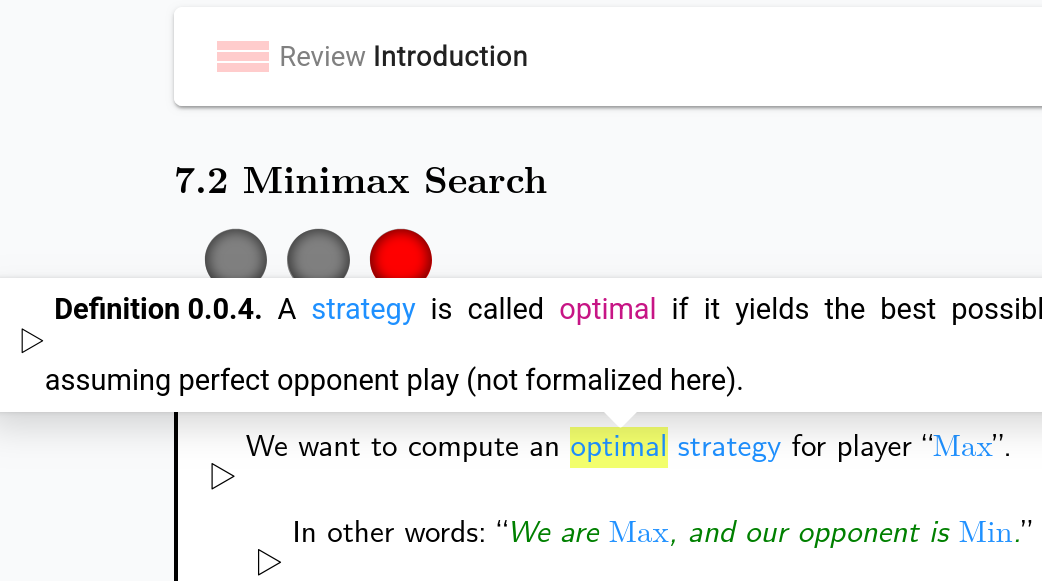
\includegraphics[width=\textwidth]{alea1.png}
    \end{columns}
\end{frame}

\begin{frame}[fragile]
    \frametitle{The cost of adoption}
    \centering
    {\bf More semantic annotations $\bm\leadsto$ better service}

    % horizontal line
    \noindent\rule{\textwidth}{0.8pt}
    \lstset{escapeinside={<*}{*>}}
%     \begin{lstlisting}
%     \textbf{Note:} Depth-limited minimax requires an
%     evaluation for every cut-off state $s$.
%     \end{lstlisting}
    % If $s$ is terminal, we use its utility, and otherwise an estimate.
    \def\h#1{\colorbox{yellow!50!red!70}{#1}}
    \begin{lstlisting}
    <*\only<2->{\h{\textbackslash usemodule[courses/FAU/AI/course]\{search/slides?id-search\}}}*>
    <*\only<3->{\h{\textbackslash usemodule[courses/FAU/AI/course]\{game-play/slides?minimax-algo\}}}*>
    \textbf{Note:} <*\only<2->{\h{\textbackslash sr\{depth limit\}\{}}*>Depth-limited<*\only<2->{\h{\}}}*> <*\only<3->{\h{\textbackslash sn\{}}*>minimax<*\only<3->{\h{\}}}*>
    requires an evaluation for every cut-off state $s$.
    If $s$ is terminal, we use its utility, and otherwise an estimate.
    \end{lstlisting}
\end{frame}

\begin{frame}
    \frametitle{Introducing snify}
    Simple tool for sTeX bulk annotation:
    \begin{itemize}
        \item Command line interface
        \item Iterates over source files
        \item Suggests annotations to user
        \item Inspired by traditional spell-checkers (e.g. ispell/aspell/...)
    \end{itemize}
\end{frame}

\begin{frame}
    \frametitle{Demo}
\end{frame}

\begin{frame}[fragile]
    \frametitle{The Catalog}
    \lstset{escapeinside={<*}{*>}}
    \def\h#1{\colorbox{yellow!70!red!70}{#1}}
    \begin{lstlisting}
... is called a \definame{<*\h{goal state}*>} (or \definiendum{goal state}{<*\h{terminal state}*>}).
    \end{lstlisting}
    \[\downarrow\text{\bf Extract verbalizations}\]
    \vspace{-1.5em}
    \begin{itemize}
        \item {\color{blue}\verb|https://...search problem&s=goal state|} $\leftrightsquigarrow$ ``goal state'', ``terminal state'', \pause ``goal'', ``end state'', ``terminal'', ``terminal positions''
        \item {\color{blue}\verb|https://...grammar&s=terminal symbol|} $\leftrightsquigarrow$ ``terminal symbol'', ``terminal''
        \item {\color{blue}\verb|https://...terminal&s=terminal|} $\leftrightsquigarrow$ ``computer terminal'', ``terminal''
        \item \textellipsis
    \end{itemize}
    \pause
    \par\vspace{1em}
    \begin{columns}
        \column{0.3\textwidth}
    \textbf{Using a stemmer to manage inflection:}
        \column{0.6\textwidth}
    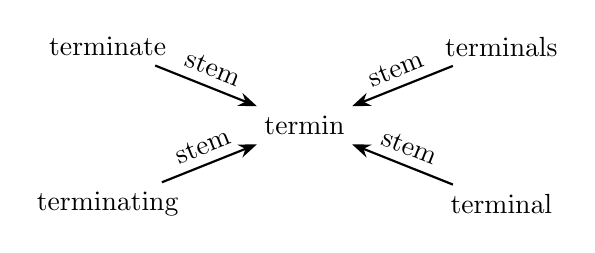
\begin{tikzpicture}
        \node (a) at (0, 0) {termin};
        \node (b) at ( 2.5, -1) {terminal};
        \node (c) at ( 2.5,  1) {terminals};
        \node (d) at (-2.5,  1) {terminate};
        \node (e) at (-2.5, -1) {terminating};
        \draw[-Stealth,thick] (b) to[sloped] node[above] {stem} (a);
        \draw[-Stealth,thick] (c) to[sloped] node[above] {stem} (a);
        \draw[-Stealth,thick] (d) to[sloped] node[above] {stem} (a);
        \draw[-Stealth,thick] (e) to[sloped] node[above] {stem} (a);
    \end{tikzpicture}
    \hfill
    \end{columns}
\end{frame}



\begin{frame}
    \frametitle{Engineering}
    \begin{itemize}
        \item Support multiple language
        \item Add new imports, remove redundant imports
        \item Only annotate text (not macros, formulae, code, \textellipsis)
    \end{itemize}
\end{frame}

\begin{frame}
    \frametitle{Productivity Features}
\end{frame}

\begin{frame}
    \frametitle{Impact}
\end{frame}

\begin{frame}
    \frametitle{Semantic Authoring}
\end{frame}

\begin{frame}
    \frametitle{Other Authoring Support}
\end{frame}

\begin{frame}
    \frametitle{Conclusion}
\end{frame}

\begin{frame}[allowframebreaks,t]
    \frametitle{References}
    \printbibliography
\end{frame}

\end{document}
